\documentclass[a4paper]{article}
\usepackage{student}
\usepackage{graphicx}
\usepackage{mathrsfs}
\usepackage{cancel}

% Metadata
\date{\today}

%-------------------------------%
% Other details
% TODO: Fill these
%-------------------------------%
\title{Taller 2}
\setmembername{Laura Rodríguez,Cristian Peña,Daniel Pardo,Miguel Martínez,Cristian Perez} 

%-------------------------------%
% Add / Delete commands and packages
% TODO: Add / Delete here as you need
%-------------------------------%
\usepackage{amsmath,amssymb,bm}
\usepackage[spanish]{babel}

% Custom your usual commands here. Renew these.
\newcommand{\KL}{\mathrm{KL}}
\newcommand{\R}{\mathbb{R}}
\newcommand{\E}{\mathbb{E}}
\newcommand{\T}{\top}
\newcommand{\expdist}[2]{%
        \normalfont{\textsc{Exp}}(#1, #2)%
    }
\newcommand{\expparam}{\bm \lambda}
\newcommand{\Expparam}{\bm \Lambda}
\newcommand{\natparam}{\bm \eta}
\newcommand{\Natparam}{\bm H}
\newcommand{\sufstat}{\bm u}

% Main document
\begin{document}
    % Add header
    \header{}

    % Use `answer` environment to add solutions
    % \begin{answer}[Question 1.1] for example starts an environment formatted
    % for Question 1.1
    15. Demostrar directamente que la transformación
$$
\begin{gathered}
Q=\arctan \frac{\alpha q}{p}, \\
P=\frac{\alpha q^2}{2}\left(1+\frac{p^2}{\alpha^2 q^2}\right)
\end{gathered}
$$
es canónica, donde $\alpha$ es una constante.
    \begin{answer}[Problema 1]
       Sean en  $(p,q)$ la coordenadas generalizadas de un sistema en el espacion de fase, y sea $H(p,q)$ la funcion de Hamilton, entonces las ecuaciones de Hamilton son:
        
        \begin{align*}
            \dot p &= -\frac{\partial H}{\partial q}, \quad \dot q = \frac{\partial H}{\partial p} \quad \text{y} \quad  \frac{\partial H}{\partial t} =0  \quad (15.1)
        \end{align*}

        Dado que la transformacion puntual de coordenadas generalizadas $(p,q)$ a coordenadas generalizadas $(P,Q)$ dada por:
        \begin{equation*}
            \begin{align*}  
                Q&=\arctan \frac{\alpha q}{p}, \\
                P&=\frac{\alpha q^2}{2}\left(1+\frac{p^2}{\alpha^2 q^2}\right) = \frac{1}{2}\left(\alpha q^2 + \frac{p^2}{\alpha} \right)
            \end{align*} \quad (15.2)
        \end{equation*}
      
        es canónica, entonces deben satisfacer las ecuaciones de Hamilton (15.1) con $K(P,Q) = K$ constante, es decir:
        \begin{align*}
            \dot P &= -\frac{\partial K}{\partial Q} \quad \text{y} \quad \dot Q = \frac{\partial K}{\partial P}  \quad \text{y} \quad \frac{\partial K}{\partial t} =0  \quad (15.3)
        \end{align*}

        Para mostrar esto ultimo, usando la regla de la cadena en la ecuaciones (15.2) y reemplazando (15.1)
        \begin{align*}
            \frac{dQ}{dt} &= \frac{\partial Q}{\partial q} \frac{dq}{dt} + \frac{\partial Q}{\partial p} \frac{dp}{dt}\\
            & = -\frac{\alpha q}{p^2 + \alpha^2 q^2} \left( -\frac{\partial H}{\partial q} \right) + \frac{\alpha p}{p^2 + \alpha^2 q^2} \left( \frac{\partial H}{\partial p} \right)\\
            &= \frac{\alpha}{p^2 + \alpha^2 q^2} \left( q\frac{\partial H}{\partial q} + p \frac{\partial H}{\partial p} \right)\\
            &= \frac 12\frac{2\alpha }{p^2 + \alpha^2 q^2} \left( q\frac{\partial H}{\partial q} +  p \frac{\partial H}{\partial p} \right)\\
            &= \frac 1 {2P}  \left( q\frac{\partial H}{\partial q} +  p \frac{\partial H}{\partial p} \right) \quad (15.4.1)
        \end{align*}
        \begin{align*}
            \frac{dP}{dt} &= \frac{\partial P}{\partial q} \frac{dq}{dt} + \frac{\partial P}{\partial p} \frac{dp}{dt}\\
            &=  \frac{p}{\alpha} \left( -\frac{\partial H}{\partial q} \right) + q\alpha\left( \frac{\partial H}{\partial p} \right) \quad (15.4.2)
        \end{align*}

        Ahora expresando $p= p(Q,P)$ y $q = q(Q,P)$:

        \begin{align*}
            \frac q p = \frac 1 \alpha \tan(Q) \quad &\Rightarrow \quad  \frac{q^2}{p^2} = \frac 1 {\alpha^2} \tan^2(Q)\\
            &\Rightarrow \quad  \frac{p^2}{\alpha^2 q^2} = \frac 1 {\tan^2(Q)}\\
            & \Rightarrow \quad  P = \frac{\alpha q^2}{2}\left(1+\frac{p^2}{\alpha^2 q^2}\right) = \frac{\alpha q^2}{2}\left(1+ \frac{1}{\tan^2(Q)} \right)\\
            & \Rightarrow \quad  q = \sqrt{
                \frac{2 P}{\alpha}}\sin (Q) \quad \text{y} \quad p = \sqrt{
                    2 P \alpha}\cos (Q) \quad (15.5)
        \end{align*}

        Y aplicando la regla de la cadena en (15.3) y reemplazando (15.5) tenemos que:
        \begin{align*}
            \dot P &= -\frac{\partial K}{\partial Q} = -\frac{\partial K}{\partial q} \frac{\partial q}{\partial Q} - \frac{\partial K}{\partial p} \frac{\partial p}{\partial Q}\\
            &=  -\frac{\partial K}{\partial q}\left( \sqrt{
                \frac{2 P}{\alpha}}\cos (Q) \right) - \frac{\partial K}{\partial p} \left( -\sqrt{
                    2 P \alpha}\sin (Q) \right)\\
            &= -\frac{\partial K}{\partial q}\sqrt{
                \frac{2 P}{\alpha}}\cos (Q) + \frac{\partial K}{\partial p} \sqrt{
                    2 P \alpha}\sin (Q) \quad (15.6.1)
        \end{align*}

        \begin{align*}
            \dot Q = \frac{\partial K}{\partial P} &= \frac{\partial K}{\partial q} \frac{\partial q}{\partial P} + \frac{\partial K}{\partial p} \frac{\partial p}{\partial P}\\
            &= \frac{\partial K}{\partial q}\left(\sqrt{\frac{1}{2Pa}} \sin (Q)\right) + \frac{\partial K}{\partial p} \left( \sqrt{\frac{a}{2P}} \cos (Q)\right) \quad (15.6.2)
        \end{align*}

        Igualando (15.4.1) con (15.6.1) y (15.4.2) con (15.6.2) tenemos que:

        \begin{align*}
            \frac 1 {2P}  \left( q\frac{\partial H}{\partial q} +  p \frac{\partial H}{\partial p} \right) &= -\frac{\partial K}{\partial q}\sqrt{
                \frac{2 P}{\alpha}}\cos (Q) + \frac{\partial K}{\partial p} \sqrt{
                    2 P \alpha}\sin (Q)\\
        \end{align*}

        Aplicando la regla de la cadena en (15.1) tenemos que:
        \begin{align*}
            \dot p = -\frac{\partial H}{\partial q} &= -\frac{\partial H}{\partial Q} \frac{\partial Q}{\partial q} - \frac{\partial H}{\partial P} \frac{\partial P}{\partial q}\\
            &= -\frac{\partial H}{\partial Q} \frac{\alpha p}{p^2 + \alpha^2 q^2}  - \frac{\partial H}{\partial P} \alpha q \quad (15.7.1)
        \end{align*}

        \begin{align*}
            \dot q = \frac{\partial H}{\partial p} &= \frac{\partial H}{\partial Q} \frac{\partial Q}{\partial p} + \frac{\partial H}{\partial P} \frac{\partial P}{\partial p}\\
            &= -\frac{\partial H}{\partial Q} \frac{\alpha q}{p^2 + \alpha^2 q^2}  + \frac{\partial H}{\partial P} \frac p\alpha \quad (15.7.2)
        \end{align*}

       

    Reemplazando (15.5) en (15.7.1) y (15.7.2) tenemos que:
    \begin{align*}
        \dot Q &= \frac 1 {2P}  \left( q\frac{\partial H}{\partial q} +  p \frac{\partial H}{\partial p} \right) \\
        &= \frac 1 {2P}  \left( q\left(\frac{\partial H}{\partial Q} \frac{\alpha p}{p^2 + \alpha^2 q^2} + \frac{\partial H}{\partial P} \alpha q\right) +  p \left(-\frac{\partial H}{\partial Q} \frac{\alpha q}{p^2 + \alpha^2 q^2}  + \frac{\partial H}{\partial P} \frac p\alpha \right) \right)\\
        &= \frac 1 {2P}  \left( \frac{\partial H}{\partial Q} \frac{\alpha pq}{p^2 + \alpha^2 q^2}  + \frac{\partial H}{\partial P} \alpha q^2 - \frac{\partial H}{\partial Q} \frac{\alpha pq}{p^2 + \alpha^2 q^2} + \frac{\partial H}{\partial P} \frac{p^2}{\alpha} \right)\\
        &= \frac 1 {2P}  \left( \frac{\partial H}{\partial P} \alpha q^2 + \frac{\partial H}{\partial P} \frac{p^2}{\alpha} \right)\\
        &= \frac 1 {2P}   \frac{\partial H}{\partial P} \left(\alpha q^2 + \frac{p^2}{\alpha} \right) \\
        &= \frac 1 {2P}   \frac{\partial H}{\partial P} 2P = \frac{\partial H}{\partial P}  \\
    \end{align*}

    \begin{align*}
        \dot P &= \frac{p}{\alpha} \left( -\frac{\partial H}{\partial q} \right) + q\alpha\left( \frac{\partial H}{\partial p} \right)\\
        &= \frac{p}{\alpha} \left( -\frac{\partial H}{\partial Q} \frac{\alpha p}{p^2 + \alpha^2 q^2}  - \frac{\partial H}{\partial P} \alpha q\right) + q\alpha\left( -\frac{\partial H}{\partial Q} \frac{\alpha q}{p^2 + \alpha^2 q^2}  + \frac{\partial H}{\partial P} \frac p\alpha \right)\\
        &=  -\frac{\partial H}{\partial Q} \frac{ p^2}{p^2 + \alpha^2 q^2}  - \frac{\partial H}{\partial P} pq  -\frac{\partial H}{\partial Q} \frac{\alpha^2 q^2}{p^2 + \alpha^2 q^2}  + \frac{\partial H}{\partial P} p q\\
        &=  -\frac{\partial H}{\partial Q} \frac{ p^2 + \alpha^2 q^2}{p^2 + \alpha^2 q^2} \\
        &=  -\frac{\partial H}{\partial Q} \\
    \end{align*}

    Por lo que si $K = H(P,Q)$ entonces las anterioes ecuaciones son las ecuaciones de Hamilton (15.3) y por lo tanto la transformacion (15.2) es canónica. Vease que como $H= H(q,p)$ no depende de $t$ entonces $K = H(P,Q)$ tampoco depende de $t$, es decir $\frac{\partial K}{\partial t} = 0$.

    \end{answer}
    2. Tomando $\mathrm{U}$ como una función de P y V, obtenga las siguientes ecuaciones:

\begin{align*}
(a)&\quad \mathrm{d} Q=\left(\frac{\partial V}{\partial P}\right)_V d P+\left[\left(\frac{\partial U}{\partial V}\right)_P+P\right] d V.\\
(b)&\quad \left(\frac{\partial U}{\partial P}\right)_V=\frac{C_V \kappa}{\beta}.\\
(c)&\quad \left(\frac{\partial U}{\partial V}\right)_P=\frac{C_P}{V \beta}-P.\\    
\end{align*}
    \begin{answer}[Punto 2]
        De las ecuaciones de transformacion asociadas a al funcion generatriz $F_2 (q_j, P_j)\quad j =1,\dots n$ dadas por:
        \begin{align*}
            Q_j &= \frac{\partial F_2}{\partial P_j},\quad  p_j = \frac{\partial F_2}{\partial q_j} \quad \text{y} \quad K = H+\frac{\partial F_2}{\partial t}  \quad (16.1)
        \end{align*}
        Se tiene que:
        \begin{align*}
            &\frac{\partial F_2}{\partial t} = 0 \quad \Rightarrow \quad K = H(Q_j,P_j)\\
            &Q_j = \frac{\partial F_2}{\partial P_j} = \frac{\partial}{\partial P_j} (P_j q_j) = q_j\\
            &p_j = \frac{\partial F_2}{\partial q_j} = \frac{\partial}{\partial q_j} (P_j q_j) = P_j\\ 
        \end{align*}
        De esta forma la matriz de transformacion $M$ es tal que:
        \begin{align*}
            M = \begin{pmatrix}
                \frac{\partial Q_i}{\partial q_j} & \frac{\partial Q_i}{\partial p_j}\\
                \frac{\partial P_i}{\partial q_j} & \frac{\partial P_i}{\partial p_j}\\
            \end{pmatrix} =\begin{pmatrix}
                \mathbf 1 & 0\\
                0 & \mathbf 1\\
            \end{pmatrix} =  \begin{pmatrix}
                1 & 0 & \dots & 0\\
                0 & 1 & \dots & 0\\
                \vdots & \vdots & \ddots & \vdots\\
                0 & 0 & \dots & 1\\
            \end{pmatrix}
        \end{align*}
    \end{answer}
    3. Un mol de un gas obedece a la ecuación de estado de van der Waals:
\begin{align*}
\left(P+\frac{a}{v^2}\right)(v-b)=R T    
\end{align*}
Donde a, b y R son constantes, demuestre que
\begin{align*}
    c_p-c_v=\frac{R}{1-2 a(1-b / V)^2 / V R T}
\end{align*}
    \begin{answer}[Punto 3]
        Dado que se busca una funcion generatriz $F'= F'(q_j, p_k,Q_l,P_m,t), \quad j + k + l+m = 2n$ tal que la transformacion canonica $M$ asociada satisfaga que:
        \begin{align*}
            \mathbf{\dot X} = M \dot {\mathbf{x} }\quad (17.1)
        \end{align*}
        Donode:
        \begin{align*}
            \mathbf X = \begin{pmatrix}
                Q_j\\
                P_j\\
            \end{pmatrix} = \begin{pmatrix}
                p_j\\
                q_j\\
            \end{pmatrix},\quad \mathbf x = \begin{pmatrix}
                q_j\\
                p_j\\
            \end{pmatrix}
            \quad \text{y} \quad 
            M = \begin{pmatrix}
                \frac{\partial Q_j}{\partial q_i} & \frac{\partial Q_j}{\partial p_i}\\
                \frac{\partial P_j}{\partial q_i} & \frac{\partial P_j}{\partial p_i}\\
            \end{pmatrix}
            \quad (17.2)
        \end{align*}
        Por lo que de (17.2):
        \begin{align*}
            M = \begin{pmatrix}
                \frac{\partial Q_j}{\partial q_i} & \frac{\partial Q_j}{\partial p_i}\\
                \frac{\partial P_j}{\partial q_i} & \frac{\partial P_j}{\partial p_i}\\
            \end{pmatrix} = \begin{pmatrix}
                \frac{\partial p_j }{\partial q_i} & \frac{\partial p_j }{\partial p_i}\\
                \frac{\partial q_j }{\partial q_i} & \frac{\partial q_j }{\partial p_i}\\
            \end{pmatrix} = \begin{pmatrix}
                0 & \delta_{ij}\\
                \delta_{ij} & 0\\
            \end{pmatrix} = \begin{pmatrix}
                0 & \mathbf 1\\
                \mathbf 1 & 0\\
            \end{pmatrix} \quad (17.3)
        \end{align*}
        Vease que $M$ de (17.3) no una transformacion canonica, pues:

        \begin{align*}
            M^T J M = \begin{pmatrix}
                0 & \mathbf 1\\
                \mathbf 1 & 0\\
            \end{pmatrix}^T \begin{pmatrix}
                0 & \mathbf 1\\
                -\mathbf 1 & 0\\
            \end{pmatrix} \begin{pmatrix}
                0 & \mathbf 1\\
                \mathbf 1 & 0\\
            \end{pmatrix}
            = \begin{pmatrix}
                0 & \mathbf 1\\
                \mathbf 1 & 0\\
            \end{pmatrix} \begin{pmatrix}
                \mathbf 1 & 0\\
                0 & -\mathbf 1\\
            \end{pmatrix} = \begin{pmatrix}
                0 & -\mathbf 1\\
                \mathbf 1 & 0\\
            \end{pmatrix} \not = J
        \end{align*}
        Por lo que en su lugar se propone:
            \begin{align*}
                \mathbf X = \begin{pmatrix}
                    Q_j\\
                    P_j\\
                \end{pmatrix} = \begin{pmatrix}
                    p_j\\
                    -q_j\\
                \end{pmatrix}
                \quad \text{y} \quad 
                M = \begin{pmatrix}
                    \frac{\partial Q_j}{\partial q_i} & \frac{\partial Q_j}{\partial p_i}\\
                    \frac{\partial P_j}{\partial q_i} & \frac{\partial P_j}{\partial p_i}\\
                \end{pmatrix} \quad (17.4)
            \end{align*}
       

     Asi de (17.4):
        \begin{align*}
            M = \begin{pmatrix}
                \frac{\partial Q_j}{\partial q_i} & \frac{\partial Q_j}{\partial p_i}\\
                \frac{\partial P_j}{\partial q_i} & \frac{\partial P_j}{\partial p_i}\\
            \end{pmatrix} = \begin{pmatrix}
                \frac{\partial p_j }{\partial q_i} & \frac{\partial p_j }{\partial p_i}\\
                \frac{\partial (-q_j) }{\partial q_i} & \frac{\partial (-q_j) }{\partial p_i}\\
            \end{pmatrix} = \begin{pmatrix}
                0 & \delta_{ij}\\
                -\delta_{ij} & 0\\
            \end{pmatrix} = \begin{pmatrix}
                0 & \mathbf 1\\
                -\mathbf 1 & 0\\
            \end{pmatrix} \quad (17.5)
        \end{align*}
        Vease que $M$ de (17.5) es una transformacion canonica, pues:
        \begin{align*}
            M^T J M = \begin{pmatrix}
                0 & \mathbf 1\\
                -\mathbf 1 & 0\\
            \end{pmatrix}^T \begin{pmatrix}
                0 & \mathbf 1\\
                -\mathbf 1 & 0\\
            \end{pmatrix} \begin{pmatrix}
                0 & \mathbf 1\\
                -\mathbf 1 & 0\\
            \end{pmatrix}
            = \begin{pmatrix}
                0 & -\mathbf 1\\
                \mathbf 1 & 0\\
            \end{pmatrix} \begin{pmatrix}
                -\mathbf 1 & 0\\
                0 & -\mathbf 1\\
            \end{pmatrix} = \begin{pmatrix}
                0 & \mathbf 1\\
                -\mathbf 1 & 0\\
            \end{pmatrix} = J
        \end{align*}
        Donde las ecuaciones de transformacion canonica para $ F'= F'(q_j, p_k,Q_l,P_m,t)$, dadas por las transformaciones de Legnedre:

        
        \begin{align*}
            F(q_j, q_k, Q_l, Q_m, t)  \rightarrow F''(q_j, p_k, Q_l, Q_m, t) \quad \Rightarrow\\
        \end{align*} 
        \begin{align*}F''(q_j, p_k, Q_l, Q_m, t) &= q_k \frac{\partial F}{\partial q_k}  - F\\
            &= q_k p_k - F
        \end{align*}
        \begin{align*}
            F''(q_j,p_k,Q_l,Q_m,t) \rightarrow F'(q_j, p_k, Q_l, P_m, t) \quad \Rightarrow 
        \end{align*}
        \begin{align*}
            \quad F'(q_j,p_k,Q_l,P_m,t) &= Q_m \frac{\partial F''}{\partial Q_m}  - F''\\
            &= -Q_m \frac{\partial F}{\partial Q_m}  - q_k p_k + F \\
            &= Q_m P_m - q_k p_k + F(q_j, q_k, Q_l, Q_m, t) \quad (17.6)
        \end{align*}

        Donde de (17.6) se tiene que:

        \begin{align*}
            \frac{dF}{dt}  &=p_j \dot q_j + p_k \dot q_k - P_l\dot Q_l- P_m \dot Q_m - (H - K)\\
            &= \frac{\partial F}{\partial q_j} \dot q_j + \frac{\partial F}{\partial q_k} \dot q_k - \frac{\partial F}{\partial Q_l}\dot Q_l- \frac{\partial F}{\partial Q_m} \dot Q_m\\
            &= \frac d{dt}\left(F'(q_j, p_k, Q_l, P_m, t) + q_k p_k - Q_m P_m \right)\\
            &= \frac d{dt}\left(F'(q_j, p_k, Q_l, P_m, t) \right) + \frac d{dt}\left(q_k p_k \right) - \frac d{dt}\left(Q_m P_m \right)\\
            &= \frac d{dt}\left(F'(q_j, p_k, Q_l, P_m, t) \right) + \dot q_k p_k + q_k \dot p_k - \dot Q_m P_m - Q_m \dot P_m \quad \Rightarrow\\
        \end{align*}
        \begin{align*}
            \frac {dF'}{dt} &= p_j\dot q_j - q_k \dot p_k - P_l\dot Q_l + Q_m \dot P_m - (H-K)\\
            &= \frac{\partial F'}{\partial q_j} \dot q_j + \frac{\partial F'}{\partial p_k} \dot p_k + \frac{\partial F'}{\partial Q_l}\dot Q_l+\frac{\partial F'}{\partial P_m} \dot P_m + \frac{\partial F'}{\partial t} \quad \Rightarrow\\
        \end{align*}
        \begin{equation*}
            \begin{align*}
                p_j = \frac{\partial F'}{\partial q_j} & \qquad q_k = -\frac{\partial F'}{\partial p_k} \\\\
                P_l = -\frac{\partial F'}{\partial Q_l} & \qquad Q_m = \frac{\partial F'}{\partial P_m} \\\\
                \qquad K = H+\frac{\partial F'}{\partial t} 
            \end{align*} \quad (17.7)    
        \end{equation*}
        Reemplazando (17.4) en (17.7) tenemos que:
        \begin{align*}
            p_j = \frac{\partial F'}{\partial q_j} & \qquad q_k = -\frac{\partial F'}{\partial p_k} \\\\
            q_l = \frac{\partial F'}{\partial p_l} & \qquad p_m = -\frac{\partial F'}{\partial q_m} \\\\
            \qquad K = H+\frac{\partial F'}{\partial t}
        \end{align*}
    Si consideramos $F'(q_j, p_k, Q_l, P_m, t) = F^{q}_j(q_j)F^{p}_k(p_k)F^{Q}_l(Q_l)F^{P}_m(P_m)F^t(t)$ entonces:
    \begin{align*}
        p_j = \frac{dF^q_j}{dq_j} & \qquad q_k = -\frac{dF^p_k}{dp_k} \\\\
        q_l = \frac{dF^p_l}{dp_l} & \qquad p_m = -\frac{dF^q_m}{dq_m} \\\\
        \qquad K = H+\frac{dF^t}{dt}
    \end{align*}
    Ecuaciones las cuales tiene como solucion:
    \begin{align*}
        F^q_j(q_j) &= \int p_j dq_j = p_jq_j + c_1\\
        F^p_k(p_k) &= -\int q_k dp_k = - p_k q_k + c_2\\
        F^Q_l(Q_l) &= \int P_l dQ_l = P_lQ_l + c_3\\
        F^P_m(P_m) &= -\int Q_m dP_m  = -P_m Q_m + c_4\\
        F^t(t) &= \int (K-H) dt\\
    \end{align*}
    Por lo que una funcion generatriz que satisface (17.4) es
    \begin{align*}
        F'(q_j, p_k, Q_l, P_m, t) = (p_j q_j + c_1)(- p_k q_k + c_2)(P_l Q_l + c_3)(-P_m Q_m + c_4) F^t(t)
    \end{align*}
    \end{answer}
    4. La ecuación de estado de un sólido monoatómico es
$$
P v+f(v)=\Gamma u \quad (4.1)
$$
donde $v$ es el volumen molar, $\Gamma$ es la constante de Grüneisen y u es la energía interna molar debida a las vibraciones de la red. Demostrar que
$$
\Gamma=\frac{\beta v}{c_V \kappa}
$$
donde $\kappa$, es la compresibilidad isotérmica. Esta ecuación, conocida como relación de Grüneisen, juega un papel importante en la teoría del estado sólido.
    \begin{answer}[Punto 4]
        Dado que la ecuacion de estado representa un sistema hidrostatico con $u = u(P,v)$ entonces:

        \begin{align*}
            du = \left( \frac{\partial u}{\partial P} \right)_v dP + \left( \frac{\partial u}{\partial v} \right)_P dv \quad (4.2)
        \end{align*}
        Donde de (4.1):
        \begin{align*}
            \left(\frac {\partial u}{\partial P}\right)_v &= \left(
                \frac{\partial}{\partial P} \left(  P\frac v\Gamma + \frac{f(v)}\Gamma \right)
            \right)_v \\ 
            &= \frac{v}{\Gamma} 
        \end{align*}
        \begin{align*}
            \left(\frac {\partial u}{\partial v}\right)_P &= \left(
                \frac{\partial}{\partial v} \left(  P\frac v\Gamma + \frac{f(v)}\Gamma \right)
            \right)_P\\
            &= \left( \frac{\partial}{\partial v} \left( \frac{f(v)}\Gamma \right) \right)_P + \frac P \Gamma\left( \frac{\partial}{\partial v} \left(  v \right) \right)_P\\
            &= \frac 1\Gamma \left( \frac{\partial f(v)}{\partial v} \right)_P + \frac P \Gamma\\
        \end{align*}
        Reemplazando en (4.2) tenemos que:
        \begin{align*}
            \Gamma dU = v dP + \left( \frac{\partial f(v)}{\partial v} \right)_P dv + P dv \quad  &\Rightarrow \quad \left(\frac {\partial u}{\partial T}\right)_v = \frac v\Gamma \left( \frac{\partial P}{\partial T} \right)_v = c_V\\
            &\Rightarrow \quad c_V =- \frac v\Gamma \left( \frac{\partial P}{\partial v } \right)_T \left( \frac{\partial v}{\partial T} \right)_v\\
            &\Rightarrow \quad c_V = \frac v\Gamma \frac \beta \kappa \\
            &\Rightarrow \quad \Gamma = \frac{\beta v}{c_V \kappa}
        \end{align*}
       
    \end{answer}
    5. En el caso de un gas paramagnético, derive la ecuación
$$
dQ=\left(\frac{\partial U}{\partial T}\right)_{V, \mathscr{M}} d T+\left[\left(\frac{\partial U}{\partial V}\right)_{\mathscr{M}, T}+P\right] d V+\left[\left(\frac{\partial U}{\partial \mathscr{M}}\right)_{T, V}-\mu_0 \mathscr{H}\right] d \mathscr{M}
$$
    \begin{answer}[Punto 5]
        Dado que este es este es un sistema hidrostatico y paramagnetico la primera ley de la termodinamica toma la forma:
        \begin{align*}
            dQ = dU - PdV + \mu_0 \mathscr Hd\mathscr{M} \quad (5.1)
        \end{align*}
        Donde las variables termodinamicas asociadas a un sistema hidrostatico son $T,~P,~V$ y las variable termodinamicas asociadas a un sistema paramagnetico son $T, \mathscr{H}, \mathscr{M}$.
        Coordenadas de las cuales solo tres son independientes, siendo las mas convinientes $T,V,\mathscr M$, por lo tanto 
        $$dU = dU(T,V, \mathscr{M}) =  \left(\frac{\partial U}{\partial T}\right)_{V, \mathscr{M}} dT +\left(\frac{\partial U}{\partial V}\right)_{T, \mathscr{M}} dV + \left(\frac{\partial U}{\partial \mathscr{M}}\right)_{T,V} d\mathscr{M}$$ 

        Reemplazando el diferencial de energia interna en (5.1) entonces:

        \begin{align*}
            dQ &=  \left(\frac{\partial U}{\partial T}\right)_{V, \mathscr{M}} dT +\left(\frac{\partial U}{\partial V}\right)_{T, \mathscr{M}} dV + \left(\frac{\partial U}{\partial \mathscr{M}}\right)_{T,V} d\mathscr{M} - PdV + \mu_0 \mathscr H d\mathscr M\\
             &= \left(\frac{\partial U}{\partial T}\right)_{V, \mathscr{M}} dT + \left[\left(\frac{\partial U}{\partial V}\right)_{T, \mathscr{M}} - P \right]dV + \left[\left(\frac{\partial U}{\partial \mathscr{M} } \right)_{T,V} + \mu_0\mathscr H\right] d\mathscr M
        \end{align*}
    \end{answer}
    6. Demuestre que el calor transferido durante un proceso cuasiestático infinitesimal de un gas ideal se puede escribir
$$
\mathrm{d} Q=\frac{C_V}{n R} V d P+\frac{C_P}{n R} P d V
$$
Aplicando esta ecuación a un proceso adiabático, demuestre que $P V^{\gamma}=$ const.
    \begin{answer}[Punto 6]
        Dado que la ecuacion de estado para un gas ideal es:
        \begin{align*}
            PV = nRT \quad (6.1) \quad \text{con}  \quad \left(\frac{\partial U}{\partial V}\right)_T = 0 \quad \text{y} \quad \left(\frac{\partial U}{\partial P}\right)_V = 0
        \end{align*}
        Por lo que la energia interna cumple que $U = U(T)$
        \begin{align*}
            dU = \left(\frac{\partial U}{\partial T}\right)_V dT   \quad \Rightarrow \quad C_V =  \frac{dU}{dT}= \left(\frac{\partial U}{\partial T}\right)_V \quad (6.2)
        \end{align*}\
        Por otro lado de la primera ley de la termodinamica para el gas ideal, desde las ecuacion (2.1) y (6.2), toma la forma:
        \begin{align*}
            dQ = \left(\frac{\partial U}{\partial T}\right)_V dT + PdV  = C_VdT + PdV \quad (6.3)
        \end{align*}
        Donde 
        \begin{align*}
            dT &= \left(\frac{\partial T}{\partial V}\right)_P dV + \left(\frac{\partial T}{\partial P}\right)_V dP\\
            &= \frac{P}{nR}dV + \frac{V}{nR}dP \quad 
        \end{align*}
        Reemplazando en (6.3) tenemos que:
        \begin{align*}
            dQ = C_V \left( \frac{P}{nR}dV + \frac{V}{nR}dP \right) + PdV \quad &\Rightarrow \quad dQ = \frac{C_V}{nR}PdV + \frac{C_V}{nR}VdP + PdV\\
            &\Rightarrow \quad dQ = \frac{C_V}{nR}VdP + \left( \frac{C_V}{nR} + 1 \right)PdV\\
            &\Rightarrow \quad dQ =  \frac{C_V}{nR}VdP + \left( \frac{C_V + nR}{nR}\right)PdV\\
            &\Rightarrow \quad dQ =  \frac{C_V}{nR}VdP +  \frac{C_P}{nR} PdV \quad (6.4)\\
        \end{align*}
        Donde se uso que $C_P - C_V = nR$ para un gas ideal.
        Ahora si consideramos tambien que es gas esta sometido a un proceso adiabatico entonces de (6.4)
        \begin{align*}
            dQ = 0 \quad &\Rightarrow \quad \frac{C_V}{nR}VdP +  \frac{C_P}{nR} PdV = 0\\
            &\Rightarrow \quad \frac{C_V}{nR}VdP = - \frac{C_P}{nR} PdV\\
            &\Rightarrow \quad \frac{C_P}{C_V}\frac{dV}{V} = -\frac{dP}{P}\\
            &\Rightarrow \quad \gamma \ln(V) = -\ln(P) + C\\
            &\Rightarrow \quad \ln(V^\gamma) = \ln(P^{-1}) + C\\
            &\Rightarrow \quad V^\gamma = P^{-1}e^C\\
            &\Rightarrow \quad PV^\gamma = e^C = \text{constante}\\
        \end{align*}

    \end{answer}
    7. Un mol de un sistema paramagnético ideal obedece la ley de Curie.
$$
\mathscr{M} =\frac{C_{C} \mathscr H}{T}
$$
Donde $\mathscr M$ es la magnetización y $\mathscr H$ es un campo magnético externo, con constante de Curie $C_C$. Suponga que la energía interna $U$ es función de $T$ únicamente, de modo que $\mathrm{dU}=\mathrm{C}_{\mathrm{V},\mathscr M}  \mathrm{dT}$, donde $\mathrm{C}_{\mathrm{v}, \mathscr{M}}$ es una capacidad calorífica a volumen y magnetización constantes. Demostrar que la ecuación de la familia de superficies adiabáticas es
$$
\frac{C_{V, \mathscr M}}{n R} \ln T+\ln V=\frac{\mu_0 \mathscr M^2}{2 n R C_C}+\ln A,
$$
Donde A es una constante.
    \begin{answer}[Punto 7]
        Dado que este es un sistema paramagnetico e hidrostatico  con funcion de energia interna $U = U(T)$ tal que $dU = C_{V, \mathscr{M}} dT$, entonces de el ejercicio 5 tenemos que la primera ley de la termodinamica queda:
        \begin{align*}
            dQ = C_{V, \mathscr{M}} dT + PdV - \mu_0 \mathscr{H} d\mathscr{M} \quad (7.1) \quad \text{donde } \quad \left(\frac{\partial U}{\partial V}\right)_{\mathscr{M},T} = 0 \quad \text{y} \quad \left(\frac{\partial U}{\partial \mathscr{M}}\right)_{T,V} = 0 
        \end{align*}
        Y para un proceso adiabatico $dQ = 0$ entonces de (7.1) tenemos que:
        \begin{align*}
            0 = C_{V, \mathscr{M}} dT + PdV - \mu_0 \mathscr{H} d\mathscr{M} \quad &\Rightarrow \quad C_{V, \mathscr{M}} + P\frac{dV}{dT}= \mu_0 \mathscr{H}\frac{d\mathscr{M}}{dT} \quad (7.2)\\
        \end{align*}
        Donde para un gas ideal y para un sistema paramagnetico se cumplem respectivamente que:
        \begin{align*}
            PV = nRT \quad \text{y} \quad \mathscr{M} = \frac{C_C \mathscr{H}}{T} \quad &\Rightarrow \quad V = \frac{nRT}{P} \quad \text{y} \quad \frac{d\mathscr{M}}{dT} = -\frac{C_C\mathscr H}{T^2}\\
        \end{align*}
        Reemplazando en (7.2)
        \begin{align*}
            C_{V, \mathscr{M}} + P\frac{dV}{dT}= \mu_0 \mathscr{H}\frac{d\mathscr{M}}{dT} \quad &\Rightarrow \quad \frac{nRT}{V} dV =  -\left( C_{V,\mathscr M} +  \mu_0 \mathscr H\frac{C_C\mathscr H}{T^2} \right)dT\\
            & \Rightarrow \quad \frac{nR}{V} dV + C_{V,\mathscr M}\frac{dT}{T}  +  \mu_0C_C\mathscr H^2 \frac{dT}{T^3} = 0\\ 
            & \Rightarrow \quad nR \ln(V) + C_{V,\mathscr M} \ln(T) -  \frac{\mu_0 C_C\mathscr H^2 }{2T^2}  = C\\ 
            & \Rightarrow \quad nR \ln(V) + C_{V,\mathscr M} \ln(T) -  \frac{\mathscr{M}^2 }{2 C_C}  = C \quad  \frac{\mathscr{H}^2}{T^2} = \frac{ \mathscr{M}^2}{C_C^2}\\
            & \Rightarrow \quad \frac{C_{V,\mathscr M}}{nR} + \ln(V)  = \frac{\mathscr{M}^2}{2 C_C nR} + \ln(A) \quad \text{donde } A = e^C = \text{constante}\\
        \end{align*}

    \end{answer}
    8. La figura 1 , se representa un diagrama $PV$ simplificado del ciclo de gas ideal de Joule. Todos los procesos son cuasi-estáticos y $\mathrm{C_P}$ es constante. Demuestre que la eficiencia térmica de un motor que realiza este ciclo es
$$
\eta=1-\left(\frac{P_{\mathbf{1}}}{P_2}\right)^{(\gamma-1) / \gamma}
$$
figura 1. Ciclo de gas ideal Joule

\begin{figure}[h]
    \centering
    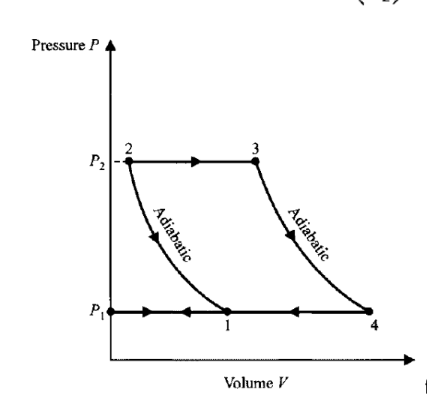
\includegraphics[width=0.5\textwidth]{diagrama.png}
    \label{fig:figura1}    
\end{figure}
    \begin{answer}[Punto 8]
        Dado que durante todo el ciclo se tiene que durante proceso isobarico se cumple
        \begin{align*}
            C_P = \left( \frac{dQ}{dT} \right)_P  \quad &\Rightarrow \quad Q_{12} = C_P \int _{T_1}^{T_2} dT = C_P (T_2 - T_1) \quad (8.1.1) \quad \text{si el calor es absorbido}\\
            &\Rightarrow \quad Q_{12} = -C_P \int _{T_1}^{T_2} dT = -C_P (T_2 - T_1) \quad (8.1.2) \quad \text{si el calor es cedido}\\
        \end{align*}
        Como de $1 \rightarrow 2$ es un proceso adiabatico entonces $dQ = 0$ y por lo tanto
        \begin{align*}
            P_1V_1^\gamma = P_2V_2^\gamma \quad (8.2)
        \end{align*}
        De $2 \rightarrow 3$ es un proceso isobarico el calor absorbido por el sistema es:
        \begin{align*}
            Q_{2\rightarrow 3} = C_P \Delta T = C_P (T_3 - T_2) \quad \text{Aplicando (8.1.1)}
        \end{align*}
        De $3 \rightarrow 4$ es un proceso adiabatico:
        \begin{align*}
            P_1V_4^\gamma = P_2V_3^\gamma \quad (8.3)
        \end{align*}
        Por ultimo de $4 \rightarrow 1$ es un proceso isocorico por lo que el calor absorbido es
        \begin{align*}
            Q_{4\rightarrow 1} = C_V \Delta T = C_P (T_4 - T_1) \quad \text{Aplicando (8.1.2)}
        \end{align*}
        Dividiendo ahora las expresiones (8.2) y (8.3) tenemos que:
        \begin{align*}
            \frac{V_1^\gamma}{V_4^\gamma} = \frac{V_2^\gamma}{V_3^\gamma} \quad &\Rightarrow \quad \frac{V_1}{V_4} = \frac{V_2}{V_3}\\
            & \Rightarrow \quad V_1 V_3 = V_2 V_4 \quad (8.4)
        \end{align*}

        Por la definicion de eficiencia:
        \begin{align*}
            \eta &= 1 - \frac{Q_{4\rightarrow 1}}{Q_{2\rightarrow 3}} = 1 - \frac{C_P (T_4 - T_1)}{C_P (T_3 - T_2)}\\
            &= 1 - \frac{T_3 - T_2}{T_4 - T_1} = 1 - \frac{\frac{P_1 V_4}{nR} - \frac{P_1 V_1}{nR}}{\frac{P_2 V_3}{nR}  -\frac{P_2 V_2}{nR}} \quad \text{Aplicando (6.1)}\\
            &= 1 - \frac{P_1V_4 -P_1 V_1 }{P_2 V_3 - P_2 V_2} = 1 - \frac{P_1}{P_2} \frac{V_3 - V_2}{V_1 - V_4}\\
            &= 1 - \left( \frac{V_2}{V_1} \right)^{\gamma} \frac{V_4 - V_1}{V_3 - V_2} = \left( \frac{V_2}{V_1} \right)^{\gamma-1} \frac{V_4V_2 - V_1V_2}{V_3V_1 - V_2V_1}  \quad \text{Aplicando (8.2)}\\
            &= 1 - \left( \frac{V_2}{V_1} \right)^{\gamma-1} \frac{ V_3 V_1 - V_2 V_1}{V_3 V_1 - V_2 V_1} = 1 - \left( \frac{V_2}{V_1} \right)^{\gamma-1} \quad \text{Aplicando (8.4)}\\
            &= 1 - \left( \frac{V_2^\gamma}{V_1^\gamma} \right)^{\frac{\gamma-1}{\gamma}} = 1 - \left( \frac{P_1}{P_2} \right)^{\frac{\gamma-1}{\gamma}} \quad \text{Aplicando (8.2)}\\
        \end{align*}
    \end{answer}
    9. (a) Deduzca la expresión para la eficiencia de un motor de Carnot directamente de un diagrama TS (Temperatura vs Entropía). (b) Compare las eficiencias de los ciclos A y B de la Figura 2.
figura 2.

\begin{figure}[h]
    \centering
    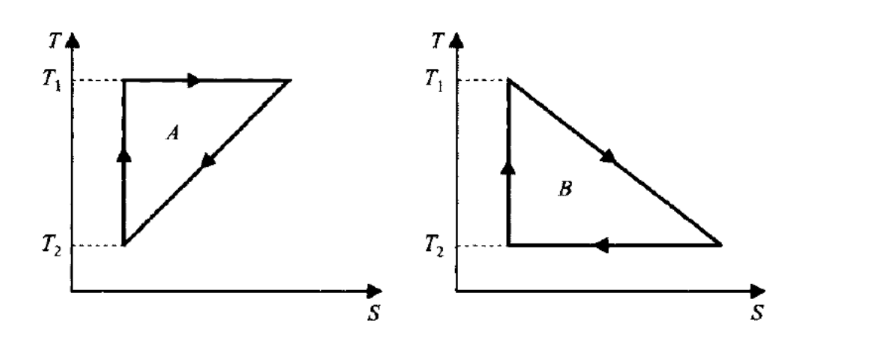
\includegraphics[width=0.5\textwidth]{diagram2.png}
    
    \label{fig:figura2}
\end{figure}
    \begin{answer}[Punto 9]
        Dado que el calor y la entropia estan relacionada por la ecuacion:
        \begin{align*}
            dQ = TdS \quad (9.1)
        \end{align*}
        \begin{itemize}
            \item [a.] En un diagrama $PV$ del un ciclo de Carnot consiste de dos curvas adiabaticas, la cuales en un digrama $TS$ consisten de dos lineas rectas que representa la entropia constante para distintos valores de la temperatura, pero a difrencia del diagrama anterior, este diagrama tambien consistira de dos curvas isotermicas representadas por dos lineas horizontales conectando las dos lineas adiabaticas, como se ve en la figura 1
            De esta manera la eficiencia va estar dada por 
    
            \begin{align*}
                \eta &= 1 - \frac{Q_{4\rightarrow 1}}{Q_{2\rightarrow 3}} = 1 - \frac{|Q_L|}{|Q_H|}\\
                &= 1 - \frac{T_L \Delta S_L}{T_H \Delta S_H} \quad \text{Aplicando (9.1)}\\
                &= 1 - \frac{T_L}{T_H} \quad 
            \end{align*}
            Esto ultimo debido a que  $2\rightarrow 3 \quad \text{y} \quad 4\rightarrow 1 \quad \text{son isoentropicos es decir} \quad S_3 = S_2 \quad \text{y} \quad S_4 = S_1 \Rightarrow \Delta S_L = \Delta S_H$
            \item [b.] Del diagrama de la izquierda obtenemos que:
            \begin{align*}
                |Q_H| &= T_1 (S_ 1- S_2)= T_1 \Delta S_H \\
                |Q_L| &= -\int_{S_1}^{S_2} T(S) dS = -\int_{S_1}^{S_2} \left( \frac{T_1 - T_2 }{S_1 - S_2}S - \frac{T_1S_2 - T_2S_1}{S_1 - S_2}\right)dS \\
                &= -\left( \frac{T_1 - T_2 }{S_1 - S_2} \frac{S_2^2 - S_1^2}{2} - \frac{T_1S_2 - T_2S_1}{S_1 - S_2} (S_2 - S_1)\right)\\
                &=-\left( T_2 - T_1 \frac{S_2 + S_1}{2} + T_1S_2 - T_2S_1\right)\\
                &= - \left(\frac 12 T_2S_1 + \frac 12 T_2 S_2 - \frac 12 T_1 S_1 - \frac 12 T_1 S_2  + T_1S_2 -T_2S_1\right)\\
                &= - \left( -\frac 12 T_1 S_1 + \frac 12 T_1 S_2 - \frac 12 T_2 S_1 + \frac 12 T_2 S_2 \right)\\
                &= - \left( \frac 12 T_1 (S_2 - S_1) + \frac 12 T_2 (S_2- S_1) \right)\\
                &= \frac 12 (T_1 + T_2) (S_1 - S_2)\\
            \end{align*}
            De esta manera la eficiencia queda:
            \begin{align*}
                \eta_L = 1 - \frac{|Q_L|}{|Q_H|} = 1 - \frac{T_1 + T_2}{2T_1} = \frac{T_1 - T_2}{2T_1}
            \end{align*}
            Ahora del  diagrama de la derecha obtenemos que:
            \begin{align*}
                |Q_L| &= T_2 (S_ 2- S_1)\\
                |Q_H| &= \int_{S_1}^{S_2} T(S) dS = \int_{S_1}^{S_2} \left( \frac{T_2 - T_1 }{S_2 - S_1}S - \frac{T_2S_1 - T_1S_2}{S_2 - S_1}\right)dS \\
                &= \left( \frac{T_2 - T_1 }{S_2 - S_1} \frac{S_2^2 - S_1^2}{2} - \frac{T_2S_1 - T_1S_2}{S_2 - S_1} (S_2 - S_1)\right)\\
                &=\left( T_2 - T_1 \frac{S_2 + S_1}{2} - T_2S_1 + T_1S_2\right)\\
                &= \left(-\frac 12 T_1S_1 - \frac 12 T_1 S_2 + \frac 12 T_2 S_1 + \frac 12 T_2 S_2  - T_2S_1 +T_1S_2\right)\\
                &= \left( -\frac 12 T_1 S_1 + \frac 12 T_1 S_2 - \frac 12 T_2 S_1 + \frac 12 T_2 S_2 \right)\\
                &= \left( \frac 12 T_1 (S_2 - S_1) + \frac 12 T_2 (S_2- S_1) \right)\\
                &= \frac 12 (T_1 + T_2) (S_2 - S_1)\\
            \end{align*}
            Por lo que ahora la eficiencia queda:
            \begin{align*}
                \eta_R = 1 - \frac{|Q_L|}{|Q_H|} = 1 - \frac{2T_2}{T_1 + T_2} = \frac{T_1 - T_2}{T_1+T_2}
            \end{align*}
            Si realizamos la difrencia de estas dos eficiencias tenemos que:
            \begin{align*}
                \eta_L - \eta_R &= \frac{T_1 - T_2}{2T_1} - \frac{T_1 - T_2}{T_1+T_2} = \frac{(T_1 - T_2)(T_1 + T_2) - 2T_1(T_1 - T_2)}{2T_1(T_1 + T_2)}\\
                &= \frac {T_1^2 - T_2^2 - 2T_1^2 + 2T_1T_2}{2T_1(T_1 + T_2)} = \frac{-T_1^2 + 2T_1T_2 - T_2^2}{2T_1(T_1 + T_2)}\\
                &= \frac{-(T_1 - T_2)^2}{2T_1(T_1 + T_2)} < 0 
            \end{align*}
            De esta forma el ciclo de la derecha es mas eficiente que el de la izquierda.

        \end{itemize}
        
    \end{answer}

    \begin{figure}[h]
        \centering
        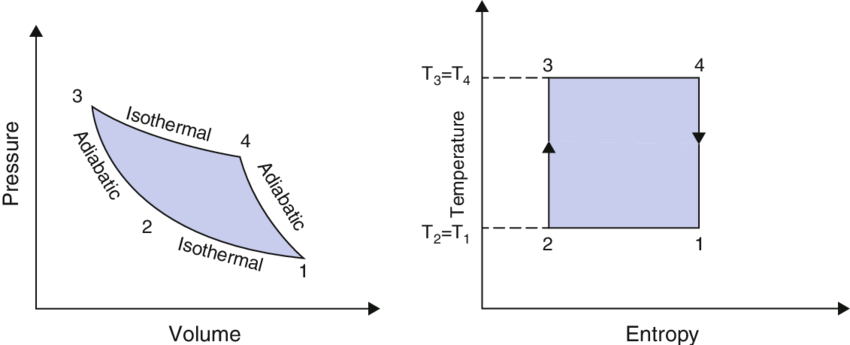
\includegraphics[width=0.5\textwidth]{Diagrama3.png}
        \caption{Diagrama $TS$ de un ciclo de Carnot}
    \end{figure}

    10. La capacidad calorífica molar a campo magnético constante de un sólido paramagnético a bajas temperaturas varía con la temperatura y el campo según la relación
$$
C_{\mathscr{H}}=\frac{B+C \mathscr{H}}{T^2}+D T^2
$$
donde B, C y D son constantes. ¿Cuál es el cambio de entropía de n moles de material cuando la temperatura cambia de $\mathrm{T_i}$ a $T_f$ mientras que $\mathscr{H}_{0}$ permanece constante en el valor $\mathscr{H_0}$ 
    \begin{answer}[Punto 10]
        La entropia esta definida por:
        \begin{align*}
            dQ = TdS \quad &\Rightarrow \quad \left( \frac{dQ}{dT}\right)_{\mathscr{H}} = T \left(\frac{dS}{dT}\right)_\mathscr{H}\\
            &\Rightarrow \quad C_{\mathscr{H}} = T \left(\frac{dS}{dT}\right)_{\mathscr{H}}\\
            &\Rightarrow \quad dS = \frac{C_{\mathscr{H}}}{T}dT\\
            &\Rightarrow \quad dS = \left(\frac{B+C \mathscr{H}_0^2}{T^2}+D T^2\right)\frac{dT}{T}\\
            &\Rightarrow \quad S = \int_{T_i}^{T_f} \left(\frac{B+C \mathscr{H}_0^2}{T^2}+D T^2\right)\frac{dT}{T}\\
            &\Rightarrow \quad S = \int_{T_i}^{T_f} \left(\frac{B+C \mathscr{H}_0^2}{T^3}+D T\right)dT\\
            &\Rightarrow \quad S = \left[-\frac{B+C \mathscr{H}_0^2}{2T^2}+D \frac{T^2}{2}\right]_{T_i}^{T_f}\\
            &\Rightarrow \quad S = -\frac{B+C \mathscr{H}_0^2}{2T_f^2}+D \frac{T_f^2}{2} + \frac{B+C \mathscr{H}_0^2}{2T_i^2}-D \frac{T_i^2}{2}\\
            &\Rightarrow \quad S = \frac{B+C \mathscr{H}_0^2}{2}\left(\frac{1}{T_i^2}-\frac{1}{T_f^2}\right)+D \left(\frac{T_f^2}{2} -\frac{T_i^2}{2}\right)\\
            &\Rightarrow \quad S = \frac{B+C \mathscr{H}_0^2}{2}\left(\frac{T_f^2 - T_i^2}{T_i^2T_f^2}\right)+D \left(\frac{T_f^2 - T_i^2}{2}\right)\\
            &\Rightarrow \quad S =\frac{T_f^2 - T_i^2}2\left[ \left(\frac{B+C \mathscr{H}_0^2}{T_i^2T_f^2}\right)+D \left(T_f^2 - T_i^2\right)\right]\\
        \end{align*}
    \end{answer}
\end{document}